\chapter{Impostazione del problema di ricerca}
\label{FormulazioneProblema}
\thispagestyle{empty}

%\begin{quotation}
%{\footnotesize
%\noindent{\emph{``Terence: Rotta a nord con circospezione \\
%Bud: Ehi, gli ordini li do io qui!\\
%Terence: Ok, comante\\
%Bud: Rotta a nord\\
%Terence: Soltanto?\\
%Bud: Con circospezione!''}
%}
%\begin{flushright}
%Chi Trova un Amico Trova un Tesoro
%\end{flushright}
%}
%\end{quotation}
\vspace{0.5cm}
In questo capitolo andiamo a descrivere, in maniera formale e rigorosa, l'ambiente e le problematiche  che l'algoritmo di tampering detection andr\`a ad affrontare. Il primo paragrafo illustra quali sono gli eventi che siamo interessati a identificare, mentre il secondo paragrafo formalizza il concetto di tampering detection.
\noindent 
\section{Modello delle osservazioni}
Il nostro campo di osservazione si concentra su quegli eventi che si interpongono tra la scena ripresa da una camera e il sensore che deve acquisire le immagini. Non vogliamo, cio\`e, identificare degli eventi particolari che avvengono nella scena, come un oggetto lasciato incustodito, bens\`i vogliamo identificare quegli eventi tali per cui il sensore non \`e pi\`u nelle condizioni di riprendere, in maniera ottimale, la scena.
Nel seguito cerchiamo di dare una definizione formale di questi eventi.
\subsection{Sfocatura}
Il fenomeno della sfocatura avviene quando un elemento trasparente o semitrasparente si interpone tra la lente della camera e la scena ripresa, causando una perdita nei dettagli della scena ripresa.

\begin{figure}
	\centering
	\includegraphics[width=6cm]{./pictures/bassiniORIGINAL}
	\includegraphics[width=6cm]{./pictures/bassiniDEFOCUS}
	\caption{Esempio di sfocatura}
	\label{fig:bassiniDEFOCUS}
\end{figure}

\noindent La figura \ref{fig:bassiniDEFOCUS} mostra un esempio di sfocatura applicata a una scena reale. 
Essa pu\`o avvenire per i pi\`u svariati motivi: 
\begin{itemize}
	\item per \textit{cause naturali}, come ad esempio dell'acqua piovana che si deposita sulla lente, oppure per la condensa dovuta all'umidit\`a e alle basse temperature, oppure un raggio di sole incidente sull'obiettivo della camera;
	\item per \textit{intervento dell'uomo}, che a sua volta pu\`o avvenire in maniera intenzionale (e in questo caso si pu\`o parlare di \textit{manomissione}) oppure non intenzionale. Ad esempio, si pu\`o direttamente intervenire sulla messa a fuoco, nel caso sia possibile cambiarla manualmente; oppure (come nel caso della figura \ref{fig:bassiniDEFOCUS}) \`e possibile applicare una sostanza semitrasparente sulla lente della camera, come il gas di un deodorante spray.
\end{itemize}
Riprendendo \cite{alippi2010detecting}, questo fenomeno pu\`o essere modellato come un operatore di \textit{degradazione} $D$ applicato a un'immagine $y$, considerata priva di errori, i.e.,
\begin{equation}
z=D[y].
\end{equation}
In particolare, all'interno dell'operatore $D$ si pu\`o considerare il contributo dovuto a un operatore di \textit{sfocatura} $B$ (dall'inglese \textit{blur}) e un termine $\eta$ corrispondente al rumore, i.e.,
\begin{equation}
\label{blur_single}
z(x)=D[y](x) = B[y](x) + \eta(x), \qquad x \in X
\end{equation}
dove abbiamo indicato con $x$ le coordinate dei \textit{pixel} dell'immagine. 
Possiamo assumere la sfocatura $B$ come un operatore \textit{lineare} di \textit{convoluzione},
\begin{equation}
B[y](x) = \int_{X}y(x)h(x,s)ds,
\end{equation}
dove $h(x,s)$ rappresenta un filtro \textit{gaussiano} o \textit{uniforme}, il cui risultato consiste nel rendere le differenze di intensit\`a, tra pixel adiacenti, pi\`u morbide (\textit{smooth}).\\
Nel caso pi\`u generale possiamo considerare che la camera acquisisca un sequenza di $N$ osservazioni $\{z_i\}, i = 1, \dots ,N$, quindi la formula \ref{blur_single} si pu\`o riscrivere come
\begin{equation}
\label{blur_multi}
z_i(x)=D[y](x) = B_i[y_i](x) + \eta(x), \qquad x \in X.
\end{equation}
La sequenza delle immagini $\{y_i\}, i = 1,\dots , N$, pu\`o variare in maniera significativa nel suo contenuto, in base alla scena ripresa.
\begin{figure}
	\centering
	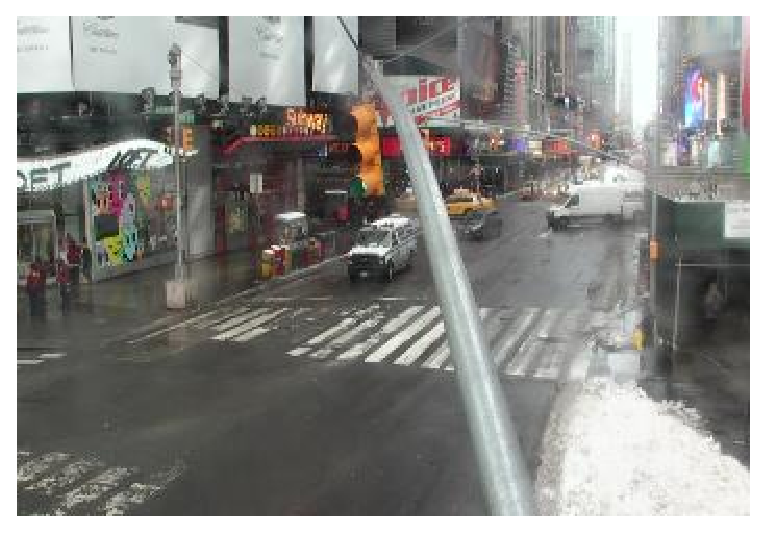
\includegraphics[width=3cm]{./pictures/image0001.eps}
	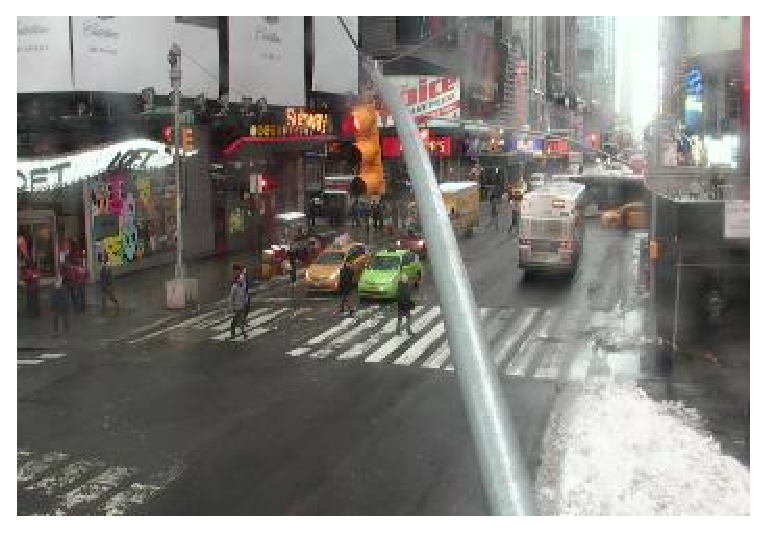
\includegraphics[width=3cm]{./pictures/image0002.eps}
	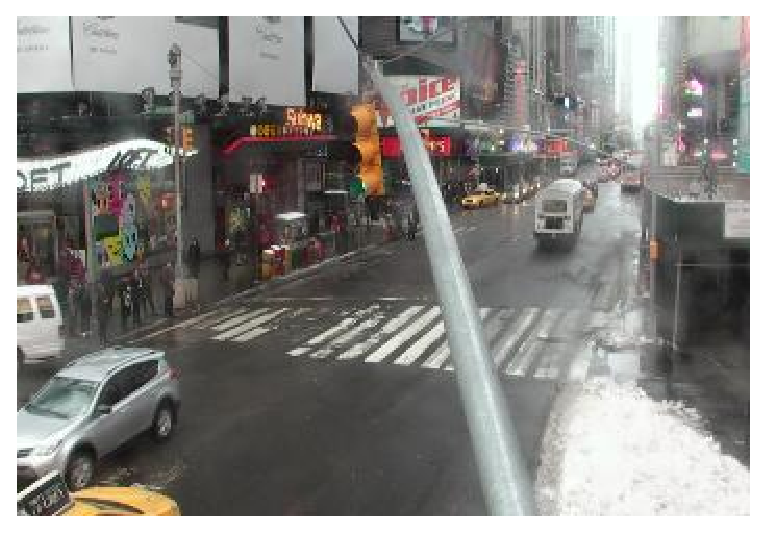
\includegraphics[width=3cm]{./pictures/image0003.eps}
	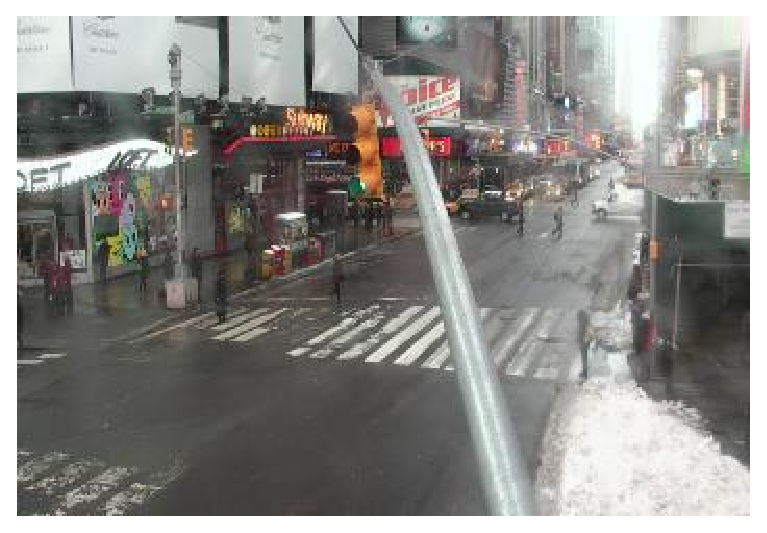
\includegraphics[width=3cm]{./pictures/image0004.eps}
	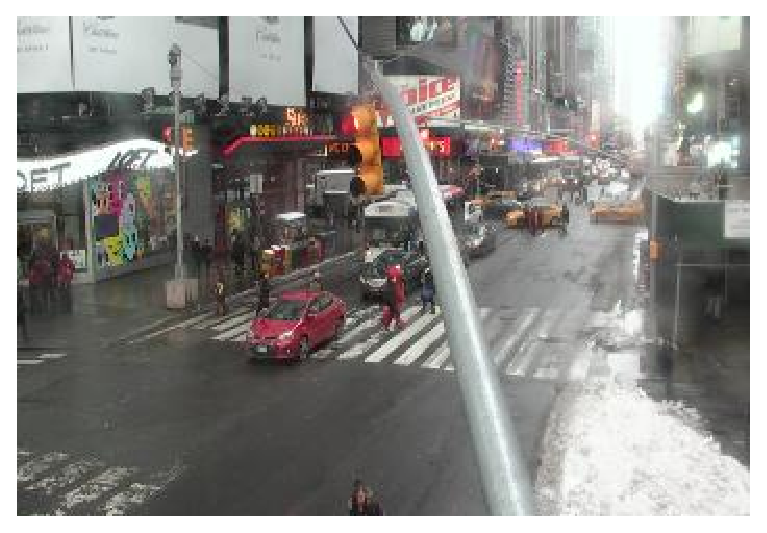
\includegraphics[width=3cm]{./pictures/image0005.eps}
	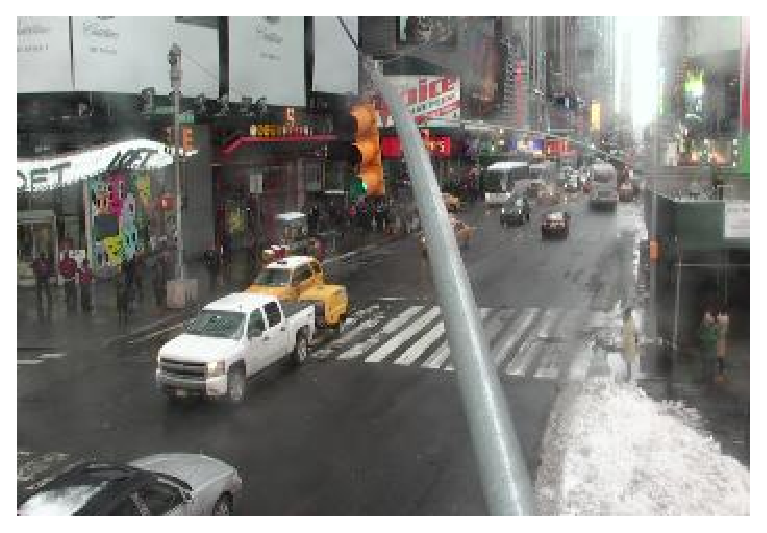
\includegraphics[width=3cm]{./pictures/image0006.eps}
	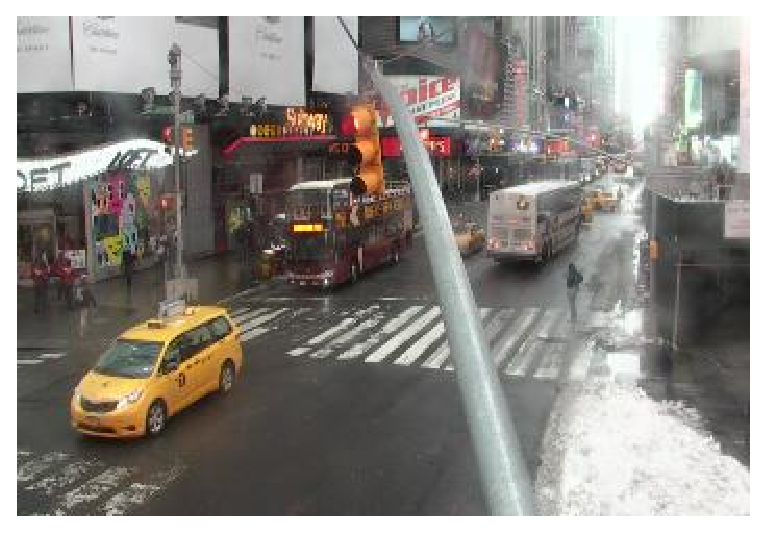
\includegraphics[width=3cm]{./pictures/image0007.eps}
	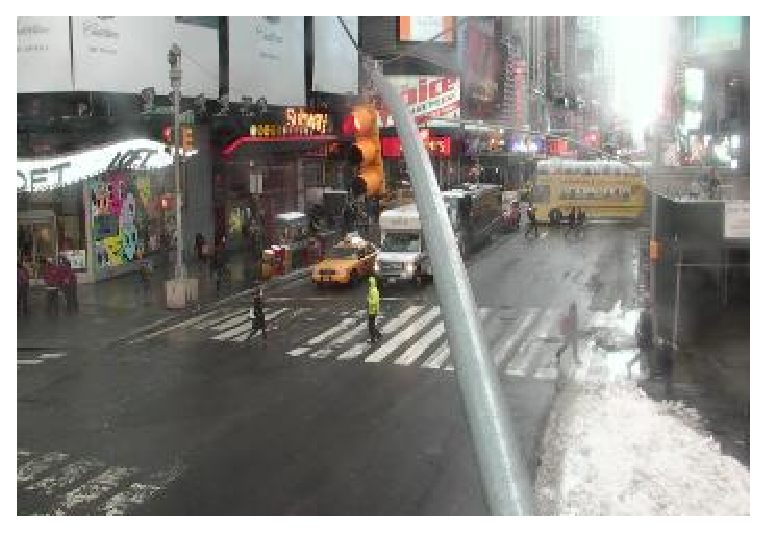
\includegraphics[width=3cm]{./pictures/image0008.eps}
	\caption{Sequenza di otto frame consecutivi acquisiti ogni minuto}
	\label{fig:framDifferences}
\end{figure}
\noindent Un esempio \`e illustrato nella figura \ref{fig:framDifferences}, in cui le immagini riprese dalla camera sono acquisite ogni minuto. 
Nonostante la scena ripresa sia la stessa, il suo contenuto varia parecchio.
Il continuo passaggio di automobili rende ciascuna immagine diversa dalle altre e, di conseguenza, usare tecniche di identificazione di cambiamenti basate sul confronto di frame consecutivi porta facilmente a un'alta generazione di falsi positivi, dato che diventa difficile distinguere il caso in cui \`e cambiato il contenuto delle immagini ($y_i \neq y_{i + 1}$) da una sfocatura ($B_i \neq B_{i + 1}$).  
\subsection{Spostamento della camera}
Lo spostamento della camera avviene quando cambia la scena ripresa.
Le cause possono essere, ancora una volta, di tipo naturale, ad esempio una raffica di vento che sposta la camera, oppure un intervento malevolo da parte di qualcuno.
\begin{figure}
	\centering
	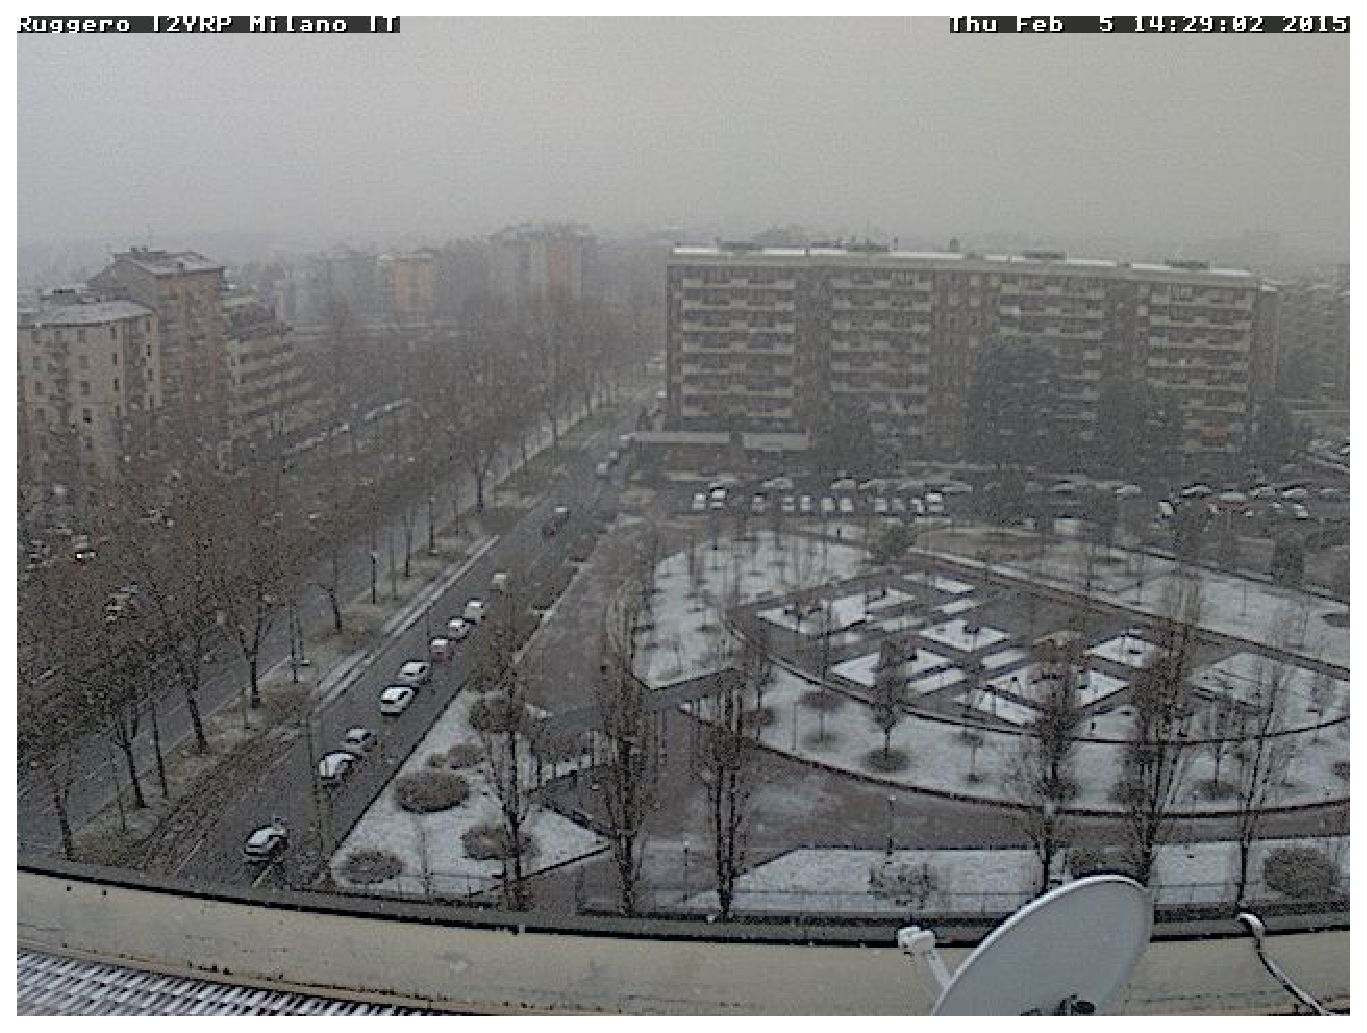
\includegraphics[width=6cm]{./pictures/testiORIGINALE}
	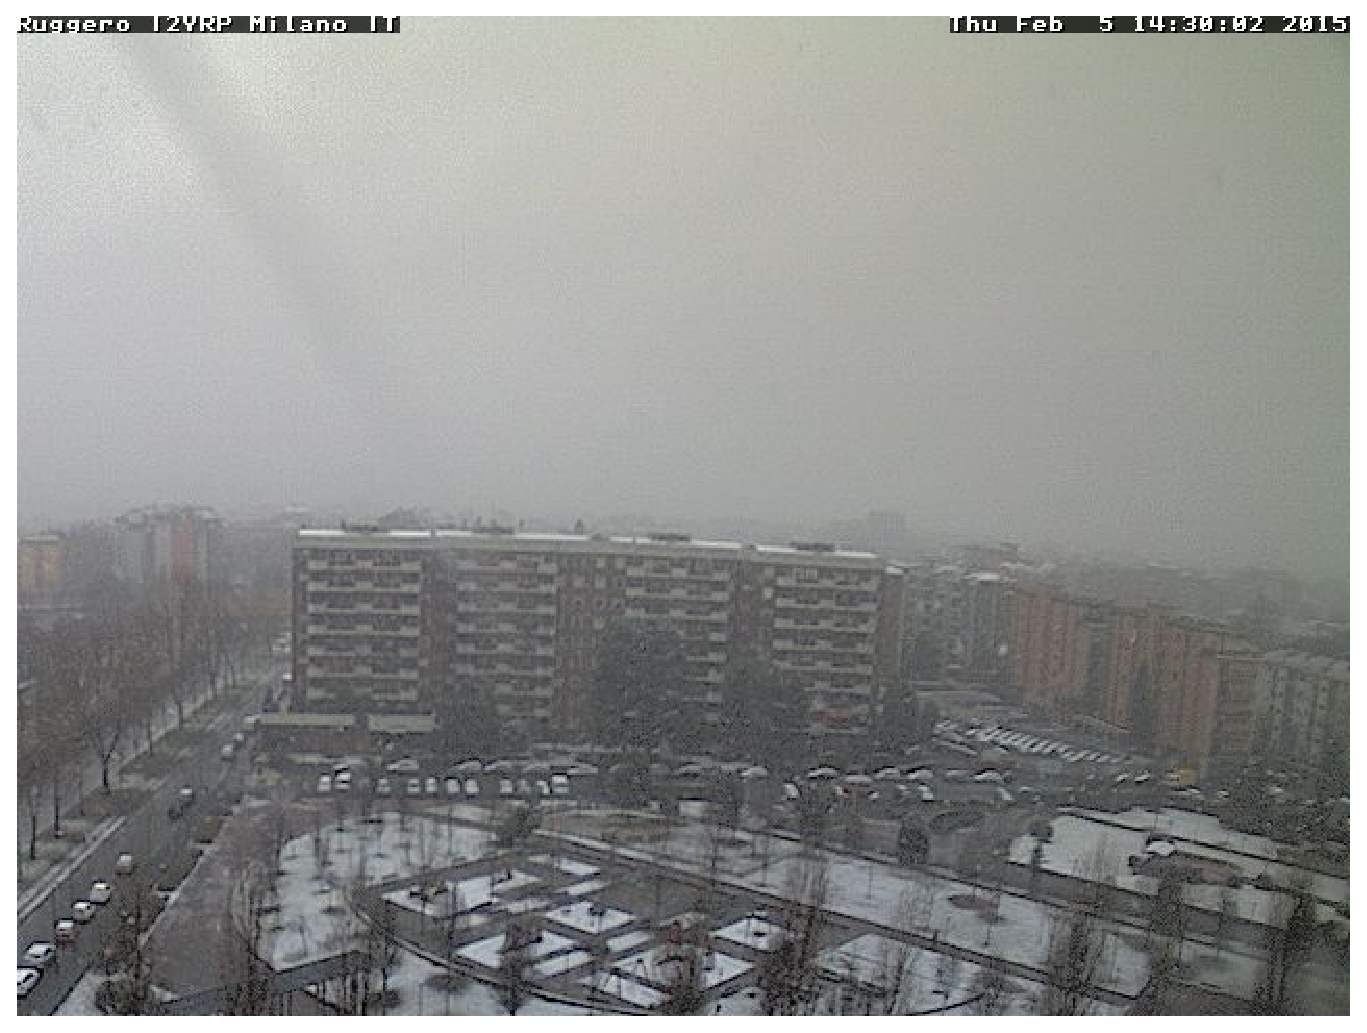
\includegraphics[width=6cm]{./pictures/testiDISPLACEMENT}
	\caption{Esempio di spostamento della camera}
	\label{fig:testiDISPLACEMENT}
\end{figure}
\noindent La figura \ref{fig:testiDISPLACEMENT} mostra un esempio di spostamento della camera tratto da un caso reale.
Possiamo formalizzare il concetto di spostamento della camera nel modo seguente: consideriamo la sequenza $\{y_i\}$ di immagini generate da una camera in una certa posizione, e la sequenza $\{w_i\}$ di immagini generate dalla stessa camera in una posizione differente.\\
Possiamo, dunque, considerare la sequenza di immagini $\{z_i\}$ in cui avviene uno spostamento della camera all'istante $T^*$ nel seguente modo:
\begin{equation}
\label{eq:displacement}
z_i(x) = \left\{ \begin{array}{rcl}
	y_i(x) + \eta(x) & \mbox{per} & i < T^* \\
	w_i(x) + \eta(x) & \mbox{per} & i \geqslant T^*,
	\end{array}\right.
\end{equation}
dove $\eta(x)$ \`e un rumore stazionario.\\
Anche per lo spostamento della camera vale la considerazione fatta nel caso della sfocatura: il contenuto delle immagini varia con il passare del tempo, quindi identificare lo spostamento confrontando frame consecutivi nel tempo genera un alto numero di falsi positivi.

\subsection{Occlusione}
\section{Tampering detection}
